\pb{TODO: source paper and contributions}



Earlier, we established that the perspective of single sample statistics is far from esoteric. In fact, anybody using a computer to analyze their data is by definition operating on a single finite bitstring. Whatever else they bring to their data is an assumption (where we will consider knowledge of the sampling process nothing but a particularly well-founded assumption).

This gives the statisticians with tabular data a comfortable corner in our worldview: they have ``assumed'' that their data can be segmented neatly into equally sized segments and that these segments have similar properties, usually because the same process generated each one independently. This is usually the most fruitful approach in single sample statistics, to take the single sample and to break it up into similarly sized pieces, in effect turning a single sample into many samples. 

Other statisticians are not so lucky. For instance, those faced with graphs: a social network, a citation network, the webgraph. These are densely interconnected objects. Following friendship links on Facebook, we can trace a path between any two random subscribers through only 3.74 intermediaries on average. Everybody is close to everybody else \cite{backstrom2012four}. This is one of the features that makes such networks so useful for things like information transfer. But it raises a question: if everybody is close to everybody else, what constitutes a ``neighbourhood''? How do we slice up the network into similar pieces? We know that social networks, at least contain clusters of friends, but finding them is no small task.

A promising approach is that of \emph{network motifs}: simply look for small subgraphs that recur frequently. These may point to communities, or to `functional units' of the network, performing the same task in different contexts. 

We investigate network motifs in Chapter~3 and show that the idea of descriptions as statistical models can be very valuable in the analysis of graphs. When we want to capture a particular structural property (like frequent occurrences of a particular subgraph) of a graph with some model, we traditional option is to create a random procedure for producing graphs, such that graphs with the required property have a high probability. 

As we've seen earlier, an equivalent approach is to simply find a description method, such that the structural property is exploited to describe the graph efficiently. We show how this principle can be applied to motif analysis, and how it allows us to massively increase the scale at which motif analysis is possible. 

We now move from the platonic world of idealized, asymptotic analysis to the mundane matter of actually analyzing real data. Our prime use case is the analysis of graph data. As we mentiond, a statistician faced with a large graph is not unlike Onno Quist: she has only one example to work with, and often very little knowledge about the process that produced the graph: how exactly are internets produced? Or social networks for that matter. In fact, one of the main research questions is usually to find the process that produced the network. Here again, the single sample setting seems not so far fetched: what assumptions, save effectiveness, can we really make to limit the model class of allowed processes? 

Since the last chapter has shown that unless our model class is highly limited, and dominating models are excluded, model selection is a hopeless business anyway, we will take a different tack. Instead of attempting to select the true model, we will use the principle of Minimum Description Length to \emph{reject} models. This will not allow us to find true pattern, necessarily, but it will provide us with patterns that \emph{might} be true. A list of candidates on  which a domain expert can build. In short we will use the principles developed so far to perform \emph{exploratory analysis}. The patterns we will focus on are \emph{network motifs}.   

\index{Exploratory analysis}\index{Network Motifs} 

\section{Introduction}

Network motifs \cite{milo2002network} provide an intuitive way to analyze graph structure. They are small, frequently occurring subgraphs. To be able to conclude that such frequent subgraphs really represent meaningful aspects of the data, we must first show that they are not simply a product of chance. That is, any subgraph may simply be a frequent subgraph in \emph{any} random graph: a subgraph is only a \emph{motif} if its frequency is \emph{higher than expected}.

This expectation is defined in reference to a \emph{null-model}: a probability distribution over graphs. We determine what the expected frequency of the subgraph is under the null-model, and if the observed frequency is substantially higher than this expectation, the subgraph is a motif. If the frequency is lower than expected, the subgraph is called an \emph{anti-motif}.

The choice of null-model is an important aspect of the analysis. Consider the case explored in \cite{carstens2013motifs}, where the data is directed and acyclic, as in the case of a citation graph. If the null model allows graph cycles, then any subgraph containing a cycle will be an \emph{anti-motif}. Such motifs show only that the data is acyclic, and obscure any deeper structure. A model that produces random acyclic graphs will fit the data better, and will allow us to explore deeper structure. This shows the role of the null-model: the better we model the \emph{known} structure in the data, the better we can expose the \emph{unknown} structure. 

However, there is usually no efficient way to compute the expected frequency of a subgraph under a null model. The most common approach is to generate a large number of random graphs, say 1000, from the null-model and compare the frequencies of the subgraph found in this sample to its frequency in the data \cite{milo2002network}. This means that any resources invested in extracting the motifs from the data must be invested again 1000 times to find out which subgraphs are motifs.

We introduce an alternative method that does not require us to repeat the motif search on samples from the null model. We use two probability distributions on graphs: the null model $p^\text{null}(G)$, and a distribution $p^\text{motif}(G)$ under which graphs with one or more frequent subgraphs have high probability. If $p^\text{motif}(G)$ is larger than $p^\text{null}(G)$, the subgraph is a motif. The section \emph{Model Selection by Codelength} explains the principle and its theoretical justification.

To design $p^\text{motif}$, we use the Minimum Description Length (MDL) Principle \cite{rissanen1978modeling,grunwald2007minimum}. It can be shown that any description method $L$, a \emph{code}, corresponds to a probability distribution $p_L$ in such a way that a graph $G$ with a short description under $L$ will have a high probability under $p_L$. This correspondence is detailed in the preliminaries. Thus, we only need to design a code that exploits recurring subgraphs to give us a probability distribution that assigns graphs with recurring subgraphs higher probability. In brief, we accomplish this by describing the motif only once, and referring back to this description wherever the motif occurs. Since we do not need to describe the motif explicitly for every occurrence, graphs with a high frequency of a certain motif will have a short description length, and thus a high probability. The code is described in the section \emph{Encoding with Motifs}.

Our method has several advantages:
\begin{itemize}
  \item The search for motifs only needs to be run once: on the data $G$. To compare the result against the null-model, we only need to know $p^\text{null}(G)$. 
  \item The number of motif instances found does not need to be an accurate estimate of the number present in the graph. The only aim is to find a sufficiently large set of non-overlapping instances in the data, to prove that the subgraph is a motif. This allows faster and simpler search algorithms to be used.
  \item Given sufficiently strong evidence, a single test can be used to eliminate multiple null models. This is explained in the section \emph{Model Selection by Codelength}.
\end{itemize}

We perform several experiments to validate these claims. First, we create random graphs with a number of occurrences of a specific subgraph inserted. We then show that our method can identify the subgraphs very precisely, even if only a small number were added. Secondly, we illustrate the behavior of the method on two directed, and two undirected graphs, using three different null models. Finally, to show what is possible with fast null models, we run the method on a dataset of a million nodes and 13 million links. This analysis was run in just under 6 hours in a single-threaded implementation, showing the scalability of the method. 

All software and data used in this paper is available. \footnote{\url{https://github.com/Data2Semantics/nodes/wiki/Motifs}} All software is released under the MIT license.

\subsection*{Related work}
Motif analysis has been applied in many domains, such as the study of biological networks \cite{wong2012biological}, the problem of community detection in social networks \cite{adamic2008knowledge} and the investigation of neural networks \cite{sporns2004motifs}. Motif extraction is a form of \emph{subgraph mining}. However, while general subgraph mining tends to focus exclusively on finding frequent subgraphs, motif extraction focuses more on the problem of finding \emph{meaningful} subgraphs, usually with the help of significance tests.  

The idea of the network motif was first introduced under that name in \cite{milo2002network}. In that paper, a computationally expensive, comprehensive search for motifs was used. Later, in \cite{kashtan2004efficient}, a simple sampling algorithm was introduced which is able find the most frequent motifs of many graphs with as little as 500 samples. However, as noted in \cite{wernicke2005faster}, it is highly biased.

A different solution to the problem of repeating the motif search on samples from the null model is provided in \cite{wernicke2005faster}: there, a faster and more correct sampling algorithm is provided, together with a technique to compute the subgraph frequencies indirectly from a single search on the data. However, this technique is restricted to the use of a specific null-model, and then only with a particular sampling method. As noted in the introduction, the restriction to one null-model is a serious drawback, and as noted in \cite{charo2010efficient}, this particular sampling method lacks strong guarantees on mixing time. \cite{ribeiro2009strategies} provides a good overview of other algorithms available for motif analysis.

The idea that compression can be used as a heuristic for subgraph discovery was also used in the SUBDUE algorithm by Cook and Holder \cite{cook1994substructure}. We introduce a compression method, connect it to the framework of motif analysis, and make the statistical implications precise.

In this paper, all candidate-motifs are induced subgraphs. This is not common to all motif analysis; in some settings the instances of the motif are allowed to have additional internal links that are not part of the motif \cite{chen2006nemofinder}. While our method could be adapted to find such motifs, it is outside the scope of the current paper.

\subsection*{Preliminaries: Graphs and Codes}
\label{section:preliminaries}

\paragraph{Graphs} A graph $G$ of size $n$ is a tuple $(N, L)$ containing a set of \emph{nodes} $N$ and a set of \emph{links} $L$. For convenience in defining probability distributions on graphs, $N$ is always the set of the first $n$ natural numbers. $L$ contains pairs of elements from $N$. Let $N_G$ be the nodeset of $G$ and $L_G$ be its linkset. For the dimensions of the graph we use the functions $n(G) = |N_G|$ and $m(G) = |L_G|$. If a graph $G$ is \emph{directed}, the pairs in $L_G$ are ordered, if it is \emph{undirected}, they are unordered. A \emph{multigraph} has the same definition as a graph, but with $L_G$ a multiset, ie. the same link can occur more than once.

A \emph{simple graph} is a graph where no link connects a node to itself. There are many types of graphs and tailoring a method to all of them is a laborious task. Here, we limit ourselves to datasets that are simple graphs. This is usually the most complex setting, so that we can trust that a method that works for simple graphs is easily translated to other settings.

Two graphs $G$ and $H$ are \emph{isomorphic} if there exists a bijection $f: N_G \to N_H$ on the nodes of $G$ such that two nodes $a$ and $b$ are adjacent in $G$ if and only if $f(a)$ and $f(b)$ are adjacent in $H$. If two graphs $G$ and $H$ are isomorphic, we say that they belong to the same isomorphism class $[G]$.

The distinction between $G$ and $[G]$ is important. Often, $G$ is given with the nodes in arbitrary order and we are actually only interested in the properties shared by all graphs in $[G]$. However, such analyses on $[G]$ can prove to be very expensive. For this reason, almost all literature on complex networks, analyzes graphs rather than isomorphism classes. Sometimes, the result is the same in both cases. For instance, let $p_a$ and $p_b$ be two graph models that are both uniform within every isomorphism class, ie. $\forall H \in [G]: p(H) = p(G)$. Then, the relative magnitude of $p_a(G)$ and $p_b(G)$ is the same as that of $p_a([G])$ and $p_b([G])$. There are other cases, however, where the analysis on $G$ must be seen as an approximation to the desired analysis on $[G]$.

\paragraph{Codes} Let $\B$ be the set of all finite-length binary strings. We use $|b|$ to represent the length of $b \in \B$. Let $\log(x) = \log_2(x)$. A \emph{code} for a set of graphs $\cG$ is an injective function $f: \cal G \to \B$. It is \emph{self-delimiting} if no code word is the prefix of another. We will denote a \emph{codelength function} with the letter $L$, ie. $L(G) = |f(G)|$. It is common practice to compute $L$ directly, without explicitly computing the codewords. In fact, we will adopt the convention of referring to $L$ itself as a code.

A well known result in information theory is the association between codes and probability distributions, implied by the  \emph{Kraft inequality}: for each probability distribution $p^*$ on $\cal G$, there exists a self-delimiting code $L^*$ such that for all $G \in \cal G$: $- \log p^*(G) \leq L^*(G) < -\log p^*(G) + 1$. Inversely, for each self-delimiting code $L^*$ for $\cal G$, there exists a probability distribution $p^*$ such that for all $G \in \cal G$: $p^*(G) = 2^{-L^*(G)}$. For proofs, see \cite[Section~3.2.1]{grunwald2007minimum} or \cite[Theorem~5.2.1]{cover2006elements}. To explain the intuition, note that we can easily transform a code $L^*$ into a sampling algorithm for $p^*$ by feeding the decoding function random bits until it produces an output. To transform a probability distribution to a code, techniques like arithmetic coding \cite{rissanen1979arithmetic} can be used. 

As explained in \cite[page 96]{grunwald2007minimum}, the discrepancy between $-\log p^*(G)$ and $L^*(G)$ can be safely ignored and we may \emph{identify} codes with probability distributions. Thus we allow $L(G)$ to take non-integer values. 

When we need to encode a single choice from a finite set $S$ of options, we will often use the code with length $\log |S|$, corresponding to a uniform probability on $S$. 

\section*{Model Selection by Codelength}

\label{section:model-selection}

The association between codes and probability distributions is particularly useful in the design of graph models: many structural properties can easily be exploited to encode a graph efficiently. Consider an undirected graph $G$ containing a large clique: all nodes in some subset $N_C \subseteq N_G$ are connected to one another directly. We can describe the graph by first describing $N_C$, and then describing $G$ in a canonical manner. Since every node in $N_C$ is connected to every other node in the clique, we can omit these links from the second part of our description, shortening the total description length, if $N_C$ is large enough. By the correspondence mentioned in the preliminaries, this gives us not just a code $L^\text{clique}$ with short codelengths for graphs with large cliques, but also a probability distribution $p^\text{clique}$ with high probabilities for graphs with large cliques. 

Of course, there is no guarantee that of all the distributions with a bias towards large cliques, $p^\text{clique}$ matches the source of our data. Luckily, it does not need to. The presence of the clique disproves the hypothesis that the data came from the null-model, so long as we can show that our clique-based model encodes the data more efficiently. Under the hypothesis that the null-model was the source of the data, we can show that the probability that any other model compresses the data better by $k$ bits or more, decays exponentially in $k$. This is known as  the \emph{no-hypercompression inequality} \cite[p103]{grunwald2007minimum}. More precisely, let $p^\text{null}(x)$ be any probability distribution, with $L^\text{null}(x) = - \log p^\text{null}(x)$ and let $L(x)$ be any code, then we have:
\[
p^\text{null}\left(L^\text{null}(x) - L(x) \geq k\right) \leq 2^{-k} \p
\]
Thus, under the null-model, the probability that $L^\text{clique}$ will compress the data better than the null-model by 10 bits or more is less than one in one-thousand. For twenty bits, we get one in a million, for thirty bits, one in a billion, and so on. So while a low codelength under $L^\text{clique}$ does not prove that the clique-code is the true model, it does allow us to comfortably reject the null model. 

We can interpret procedure as a significance test: the difference in compression $D$ between the null model and the alternative model is a statistic \cite[Example~14.2]{grunwald2007minimum}. The no-hypercompression inequality gives us a bound on the probability $p^\text{null}(D \geq k)$. To reject the null-model with significance level $\alpha$, we must find some code on the set of all graphs and show that it compresses the data better than the null-model by $k$ bits, with $2^{-k} \leq \alpha$. Any code will do, so long as it was chosen before seeing the data.

Note that $D$ is also the logarithm of the likelihood ratio between the null model and $L$, so we can see this as a likelihood ratio test. We can also interpret the difference in codelength between two models $p_a$ and $p_b$  as the logarithm of the \emph{Bayes factor} $p_a(x)/p_b(x)$ \cite[Section~14.2.3]{grunwald2007minimum}. 

Now, while our test  only \emph{rejects} the null-model, and does not confirm anything, we would like to make sure that it was the pattern we are interested in (eg. the clique) that allowed us to reject the null model, and not some other aspect of the alternative model. To ensure this, we aim to have the alternative model exploit only the pattern, and nothing else. We use the null model for everything but the pattern. For instance, in the example above, the clique model must store the graph minus the links of the clique. If we use the null model for this, we know that the only change between the null model and the alternative is the use of the clique, so that must be what made the difference.

A final benefit of this method is that we can reject multiple null models with a single test. In many situations we will have a function $B(G)$ that lower bounds any code in some set $\cal L$. If our alternative model provides a codelength below $B(G) - k_\alpha$ with $k_\alpha$ the number of bits required for our chosen $\alpha$, we can reject all of $\cal L$.

As an example, Let $\cG_n$ be the set of all undirected graphs of size $n$. We can define a uniform code on such graphs: $L^\text{uniform}_n = \log |\cG_n|$. This code captures the idea that the size of the graph is the only informative statistic: given the size, all graphs  are equally likely. This is a good null-model to test the assumption that the graph contains no significant structure, save for its size. However, it is \emph{parametrized}. It is currently not a code on \emph{all} graphs, just those of size $n$. To turn it into a code that can represent all graphs, we need to encode the parameter $n$ as well, with some code over the natural numbers
\[
L^\text{complete}(G) = L^\N(n(G)) + L^\text{uniform}_{n(G)}(G) \p
\]
This is called \emph{two-part coding}, we encode the parameters of a model first, and then the data given the parameters. For some parametrized model $L_\theta$, we can choose any code for $\theta$ to make it complete. We will call the set of all such complete codes the \emph{two-part codes on $L_\theta$}. 

Which two-part code we choose is arbitrary. We may be able to reject the uniform code for one choice of $L^\N$, or several, but how can we prove that $L^\text{complete}$ will be rejected whatever $L^\N$ we choose? Instead of choosing an arbitrary code for the size, we can instead use the \emph{bound} $B(G) = L^\text{uniform}_{n(G)}(G)$ as our null model. This is not a code, but it \emph{is} a lower bound for any two-part code on $L^\text{uniform}_n$. If $L^\text{clique}(G)$ is shorter than $B(G)$, it is also shorter than $L^\text{complete}(G)$ for any choice of $L^\N$.\footnotemark

\footnotetext{
In probabilistic terms, the code on the parameter corresponds to a prior on the parameter. The two-part codes correspond to maximum likelihood posterior probabilities: $p(\hat\theta) p(x \mid\hat\theta)$. Our bound corresponds to the maximal likelihood of the data: $p(x \mid \hat \theta)$. This shows us that the bound applies not only to the two-part codes, but also to the full mixture: $\sum_\theta p(x \mid \theta) p(\theta) \leq \sum_\theta p(x \mid \hat\theta) p(\theta) = p(x \mid\hat\theta)$
} 

Contrast this with the traditional approach, where we would define a statistic on $G$, like the size of the largest clique, and compare the observed value of the statistic with the expectation under the null model. In this case the models would have to be rejected with separate tests. If a large clique is unlikely in a sample from $p^\text{uniform}_n$, we have no guarantee that it will also be unlikely in a sample from $p^\text{complete}$. 

Note that when we store the rest of the graph within $L^\text{clique}$ we \emph{cannot} use $B(G)$ in place of $L^\text{complete}(G)$. We want a \emph{conservative} hypothesis test: the probability of rejecting a true null model may be lower than $\alpha$ but never higher. By this principle, bounds chosen in place of a model should always decrease $D$. The code corresponding to the null-model must always be lowerbounded, and the code for the alternative model must always be upperbounded. Thus when we re-use the null model inside the alternative model, we must always use a complete code.

\section*{Encoding with Motifs}

\label{section:motif-code}

Let $S = \langle S_1, \ldots, S_k \rangle$ be an ordered set of nodes from $N_G$. The \emph{induced subgraph} $I(S, G)$ is a graph $G'$ with $k$ nodes, containing a link  $(i, j)$ if and only if $G$ has a link $(S_i, S_j)$. That is, the induced subgraph extracts all links existing between members of $S$. 

Assume that we are given a graph $G$, a potential motif $G'$, and a list ${\cal M}^\text{raw} = \langle M_1, \ldots, M_k\rangle$ of instances of $G'$ in $G$. That is, each sequence $M\in {\cal M}^\text{raw}$ consists  of nodes in $N_G$, such that the induced subgraph $I(M, G)$ is equal to $G'$. Sequences in ${\cal M}^\text{raw}$ may overlap, ie. two instances may share one or more nodes. We are also provided with a generic graph code $L^\text{base}(G)$ on the simple graphs. 

The basic principle behind our code is illustrated in Fig.~\ref{figure:motif-code}: we want to store the motif only once, remove as many instances of the motif from the data as we can, and replace them with references to the stored motif. The two graphs combined contain enough information to recover the data, but we have only had to describe the motif once. Algorithm~\ref{algorithm:motif-code} describes the exact process. 

\begin{figure*}[htb]
  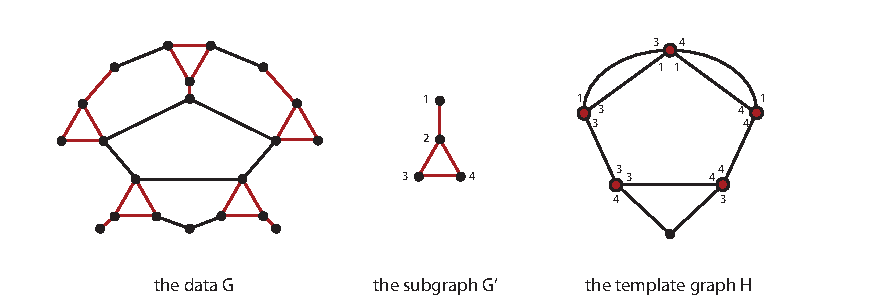
\includegraphics[width=\textwidth]{./images/illustration.pdf}
  \caption{An illustration of the motif code. We store $G'$ once, and remove its instances from $G$, replacing them with a single, special node. The links to special nodes are annotated with `rewiring' information, which tells us how to rewire the subgraph back into $H$. Storing only $H$ and $G'$ is enough to reconstruct the data.}
   \label{figure:motif-code}
\end{figure*}  

The first thing we need for this scheme is a subset $\cal M$ of ${\cal M}^\text{raw}$ such that the instances contained within it do not overlap: ie for each $M_a$ and $M_b$ in $\cal M$, we have $M_a \cap M_b = \emptyset$. Selecting the subset that would give us optimal compression is NP-Hard (as the set cover problem is reducible to it), so we must make do with an approximation. As we will see later, the most important factor is the number of links an instance has to nodes outside the instance. We call this the \emph{exdegree}.\footnote{Unlike the in- and outdegree the exdegree is not a property of a node, but of a subgraph.} In order to find a subset of instances with low exdegree, we first sort ${\cal M}^\text{raw}$ by exdegree in ascending order. We then remove the first $M$, add it to our subset $\cal M$ and remove all other instances that overlap with it. We continue removing the first remaining instance until $\cal M$ is empty.

In the following, we will often need to store a sequence of integers. We will store all such sequences using the code corresponding to a \emph{Dirichlet-Multinomial} (DM) distribution. Let $S$ be a sequence of length $k$ of elements in alphabet $\Sigma$. Conceptually, the DM distribution models the following sampling process: we sample a probability vector $p$ on $[0, |\Sigma|]$ from a Dirichlet distribution with parameter vector $\alpha$, and then sample $k$ symbols from the categorical distribution represented by $p$. The probability mass function corresponding to this process can be expressed as:
\begin{align*}
&p^\text{DirM}_\alpha(S\mid k, \Sigma) = \prod_{i \in [1,k]} \text{DirM}_\alpha(S_i\mid S_{1:i-1})  \\
&p^\text{DirM}_\alpha(S_i \mid S', k, \Sigma) = \frac{f(S_i, S') + \alpha_i}{|S'| + \sum_i \alpha_i}
\end{align*}
where $f(x, X)$ denotes the frequency of $x$ in $X$. We use $\alpha_i = 1/2$ for all $i$. Let $L^\text{DirM}_{k,\Sigma} (S) = -\log p^\text{DirM}(S \mid k, \Sigma)$. Note that this code is parametrized with $k$ and $\Sigma$. If these cannot be deduced from earlier parts of the code, they need to be encoded separately. Often, we will have $\Sigma = [0, n_\text{max}]$, and we only need to encode $n_\text{max}$.

We also require a self delimiting code to represent natural numbers. We will use the code corresponding to the probability distribution $p^\N(n) = 1/ (n(n+1))$, and denote it $L^\N(n)$.

\begin{description}
\item[subgraph] First, we store the subgraph $G'$ using $L^\text{base}(G')$ bits.
\item[template] We then create the \emph{template graph} $H$ by removing the nodes of each instance $M \in \cal M$, except for the first, which becomes a specially marked node, called an \emph{instance node}. The internal links of $M$---those incident to two nodes both in $M$---are removed from the graph. Any link connecting a node outside of $M$ to a node inside of $M$ is kept, and rewired to the instance node.
\item[instance nodes] $L^\text{base}$ does not record which nodes of $H$ are instance nodes, so we must record this separately. There are $n(G) \choose |{\cal M}|$ possibilities, so we can encode this information in $\log {n(g) \choose |{\cal M}|}$ bits.
\item[rewiring] For each side of a link in $H$ incident to an instance node, we need to know which node in the motif it originally connected to. Let there be some agreed-upon order in which to enumerate the links of any given graph. Given this order, we only need to encode the sequence $W$ of integers $w_i \in [1,\ldots, n(G')]$. We do so using the DM model described above. The maximum symbol and length of $W$ can be deduced from parts already encoded. Note that this code is invariant to the ordering of $W$, so the particulars of the canonical node ordering do not need to be specified.
\item[multiple edges] Since $L^\text{base}$ can only encode simple graphs, we cannot use it to store $H$ directly, since collapsing the instances into single nodes may have created multiple edges. In this case we remove all multiple edges and encode them separately. We assume a canonical ordering over the links and record for each link incident to an instance node, how many copies of it were removed. This gives us a sequence $R$ of natural numbers $R_i \in [0, r_\text{max}]$ which we store by first recording the maximum value in $L^\N(\max(R))$ bits, and then recording $R$ with the DM model.
\item[insertions] Finally, while $H$ and $G'$ give us enough information to recover a graph isomorphic to $G$, we cannot yet reconstruct where each node of a motif instance belongs in the node ordering of $G$. Note that the first node in the instance became the instance node, so we only need to record where to insert the rest of the nodes of the motif. This means that we perform $|{\cal M}| (n(G')-1)$ such insertions. Each insertion requires $\log (t+1)$ bits to describe, where $t$ is the size of the graph before the insertion. Let $H$ be the template graph and $G$ the complete graph, then we require $\sum_{t=n(H)}^{n(G)-1} \log (t+1) = \log (n(G)!) - \log (n(H)!)$ bits to record the correct insertions.
\end{description} 

\begin{pseudo}[th]
\caption{The motif code $L^\text{motif}(G ; G', {\cal M}, L^\text{base})$. Note that the nodes of the graph are integers.}
\label{algorithm:motif-code}
{ 
Given:\\ 
\tab a graph $G$, a subgraph $G'$,\\ 
\tab a list $\cal M$ of instances of $G'$ in $G$, a code $L^\text{base}$ on the simple graphs.\\
\\
$b_\text{subgraph} \leftarrow L^\text{base}(G')$\hfill \textbf{subgraph} \\
\\
\emph{\# replace each instance with a single node} \\
$H \leftarrow \text{copy}(G)$, $W = [] $\hfill \textbf{template} \\
\textbf{for each } $M = \{ m_1, \ldots m_{n(G')}\}$ \textbf{in} $\cal M'$:\\
\tab \emph{\# We use $m_1$ (the $m_1$-th node in $G$) as the instance node}\\
\tab \textbf{for each} link $l$ between a node $n_\text{out}$ not in $M$ and a node $m_j$ in $M$:\\
\tab \tab \textbf{if} $j \neq 1$: add a link between $n_\text{out}$ and $m_j$\\
\tab \tab $W$.append$(j)$\\
\tab remove all nodes $m_i$ except $m_1$, and all incident links\\
$b_\text{rewiring} \leftarrow  L^\text{DirM}_{|W|, n(G')}(W)\hfill\textbf{rewiring}$\\
\\
\emph{\#Remove multiple edges from $H$  and record the duplicates in $R$}\\
$R, H' \leftarrow \text{simple}(H)$ \\
$b_\text{template} \leftarrow L^\text{base}(H')$\\ 
$b_\text{multi-edges} \leftarrow L^\N(\max(R)) + L^\text{DirM}_{|R|, \max(R)}(R)$ \hfill \textbf{multiple edges}\\
\\
$b_\text{instances} \leftarrow \log {n(G) \choose |{\cal M'}|}$ \hfill \textbf{instance nodes}\\
$b_\text{insertions} \leftarrow \log (n(G))! - \log (n(H))!$ \hfill \textbf{insertions}\\    
\\
\textbf{return} $b_\text{subgraph} + b_\text{template} + b_\text{rewiring} + b_\text{multi-edges} + b_\text{instances} + b_\text{insertions}$\\
}
\end{pseudo} 

\paragraph{search} Since our code accepts any list of motif instances, we are free to take the list $\cal M$ and prune it further, before passing it to the motif compressor, effectively discounting instances of the motif. This can often improve compression, as storing the rewiring information for instances with high exdegrees may cost more than we gain from removing them from the graph. We will sort  $\cal M$ by exdegree and search for the value $c$ for which compressing the graph with only the first $c$ elements of $\cal M$ gives the lowest codelength.

The codelength $L^\text{motif}$ as a function of $c$ is roughly unimodal, which means that a ternary search should give us a good value of $c$ while reducing the number of times we have to compute the full codelength. We use a \emph{Fibonacci search} \cite{kiefer1953sequential}, an elegant variation on ternary search requiring only one sample per recursion. Note that $c$ is not a parameter of the model, so we do not need to store it separately.  

\paragraph{implementation} The \textbf{template} part of the code can be time and memory intensive for large graphs, as it involves creating a copy of the data. For any given $L^\text{base}$, we can create a specific implementation which computes the codelength required for storing the template graph without constructing $H$ explicitly. This will speed up the computation of the code at the expense of creating a new implementation for each new null model. We use such specific implementations for our three null models.

\section*{Null Models}

We will define three null models. For each model we follow the same pattern, we first describe a parametrized model (which does not represent a code on all graphs). We then use this to derive a bound as described in the second section, so that we can reject a set of null models, and finally we describe how to turn the parametrized model into a complete model to store graphs within the motif code.  

Specifically, let $L^\text{name}_\theta(G)$ be a parametrized model with parameter $\theta$. Let $\hat\theta(G)$ be the value of $\theta$ that minimizes $L^\text{name}_\theta(G)$ (the maximum likelihood parameter). From this we derive a bound $B^\text{name}(G)$ from this---usually using $B^\text{name}(G) = L^\text{name}_{\hat\theta(G)}(G)$---which we will use in place of a null-model. Finally, we create the complete model by two-part coding: $L^\text{name}(G) = L^{\theta}(\hat\theta(G)) + L^\text{name}_{\hat\theta(G)}(G)$. 

\subsection*{The Erd\H{o}s-Renyi Model}

The Erd\H{o}s-Renyi (ER) model is probably the best known probability distribution on graphs\cite{renyi1959random,gilbert1959random}. It takes a number of nodes $n$ and a number of links $m$ as parameters, and assigns equal probability to all graphs with these attributes, and zero probability to all others. This gives us 
\[
L^\text{ER}_{n, m}(G) = \log{(n^2-n)/2 \choose m} 
\] 
for undirected graphs, and 
\[
L^\text{ER}_{n, m}(G) = \log{n^2-n \choose m} 
\] 
for directed graphs. We use the bound $B^\text{ER}(G) = L^\text{ER}_{n(G), m(G)}(G)$.

For a complete code on simple graphs, we encode $n$ with $L^\N$. For $m$ we know that the value is at most $m_\text{max}=(n^2-n)/2$ in the undirected case, and at most $m_\text{max}=n^2-n$ in the directed case, and we can encode such a value in $\log m_\text{max}$ bits: 
\[
L^\text{ER}(G) = L^\N(n(G)) + \log m_\text{max} + L^\text{ER}_{n(G), m(G)}(G)\p
\]
 
\subsection*{The Degree-Sequence Model}
\label{section:degree-sequence-model}

The most common null-model in motif analysis is the \emph{degree-sequence model} (also known as the \emph{configuration model} \cite{newman2010networks}). 
For undirected graphs, we define the degree sequence of graph $G$ as the sequence $D(G)$ of length $n(G)$ such that $D_i$ is the number of links incident to node node $i$ in $G$. For directed graphs, the degree sequence is a pair of such sequences $D(G) = (D^\text{in}, D^\text{out})$, such that $D^\text{in}_i$ is the number of incoming links of node $i$, and $D^\text{out}_i$ is the number of outgoing links.

\paragraph{The parametrized model $L^\textnormal{DS}_D(G)$} The degree-sequence model $L^\text{DS}_D(G)$ takes a degree sequence $D$ as a parameter and assigns equal probability to all graphs with that degree sequence. Assuming that $G$ matches the degree sequence, we have $L^\text{DS}_D(G) = \log |\cG_D|$ where $\cG_D$ is the set of simple graphs with degree sequence $D$. There is no known efficient way to compute this value for either directed or undirected graphs, but various estimation procedures are known. We use an importance sampling algorithm discovered independently by \cite{blitzstein2011sequential} and \cite{charo2010efficient}.\footnotemark~This algorithm is guaranteed to produce any graph matching $D$ with some nonzero probability. Crucially, the algorithm does not backtrack or reject candidates, which means that if we multiply the probability of each random choice made in sampling, we get the probability of the sample under our sampling procedure. That is, the algorithm produces, along with a sample $G \in \cG_D$, the probability $q^\text{DS}_D(G)$ of the algorithm producing $G$. While the samples are not uniform, we do have:
\begin{equation}
{E} \left [\frac{1}{q^\text{DS}_D(G)}\right] = |\cG_D| \label{line:expectation}
\end{equation}
where $G$ is a random variable representing a sample from the algorithm. Thus, we can sample a number of graphs and take the mean of their inverse probability under $q^\text{DS}_D$ to estimate $p^\text{DS}_D(G)$. This is a form of \emph{importance sampling}. 

This approach was taken in \cite{blitzstein2011sequential}: the sample mean $1/n \sum_i 1/q^\text{DS}_D(G_i)$ was used as an estimator for the expectation in (\ref{line:expectation}). However, as shown in \cite{charo2010efficient}, the distribution of $1/q^\text{DS}_D(G)$ tends to be very close to log-normal. This means that the sample mean will converge \emph{very} slowly to the correct value. Specifically, the standard deviation of this estimate after $n$ samples is $\frac{1}{\sqrt{n}} \sqrt{(e^{\sigma^2}-1)e^{2\mu +\sigma^2}}$, which for a distribution with $\mu=200$ and $\sigma=10$, leads to a standard deviation of approximately $\frac{1}{\sqrt{n}} e^{300}$.

For this reason, we use the \emph{maximum-likelihood estimator} for the log-normal distribution instead. Let $Q_i = 1/q^\text{DS}_{D}(G_i)$. We assume $Q_i$ is log-normally distributed, so that $Y_i = \log Q_i$ is normally distributed. Let $\overline{Y} = \frac{1}{n}\sum_i Y_i$ and $S_Y = 1/n \sum_i (\overline{Y} - Y_i)^2$; then the maximum-likelihood estimator of $EQ$ is $\exp\left(\overline{Y} + \frac{1}{2}S_Y\right)$. Thus, the codelength under the degree sequence model can be estimated as $\left(\overline{Y} + \frac{1}{2}S_Y\right)\log_2(e)$.

\footnotetext{Specifically, our implementation uses the algorithms described in \cite{charo2010efficient} and \cite{kim2012constructing}. However the non-uniform sampling from the candidate set, discussed in \cite[p10, step 5]{blitzstein2011sequential} is crucial to achieving a low variance in the sampling distribution, and thus a fast convergence.}

Unfortunately, even with the highly optimized implementations described in \cite{charo2010efficient} and \cite{kim2012constructing} sampling can be slow for large graphs. Luckily, we are only interested in an estimate of the codelength accurate to around the level of single bits, which means that we only need to sample until we have a rough estimate of the order of magnitude of $|\cG_D|$. For instance, if we accept a margin of error of only 15 bits (of the potentially $10^6$ bits required to store the graph), we can underestimate the number of graphs by 4 orders of magnitude and still end up within the margin. All we need is a reliable confidence interval for our estimate, so that we can choose a suitably conservative bound for our estimate. Our method of obtaining such a confidence interval is described in the supporting materials. In all cases, we use a one-sided confidence interval: when computing the codelength under the null model, we use a lower bound for the true value, and when computing the codelength for the motif code, we use an upper bound. Thus, the difference in codelength is a lower bound for the true value.

\paragraph{The bound $B^\textnormal{DS}(G)$} To get a bound for all two-part codes on $L^\text{DS}_D$, we could use ${B'}^\text{DS}(G) = L^\text{DS}_{D(G)}(G)$. Beating such a bound would tell us that no property of the degree sequence could explain the motif we had found. Unfortunately, the degree sequence forms a large part of the code, and a lot of evidence is required to compress better than ${B'}^\text{DS}(G)$ with a complete code. 

Instead, we make the assumption that the degrees are sampled independently from a single distribution $p^\text{deg}(n)$ on the the natural numbers. This corresponds to a code $\sum_{D_i \in D}L^\text{deg}(D_i)$ on the entire degree sequence. Let $f(s, D)$ be the frequency of symbol $s$ in sequence $D$. It can be shown that $B^\text{deg}(D) = \sum_{D_i \in D} f(D_i, D)/|D|$ is a lower bound for any such code on the degree sequence. This gives us the bound $B^\text{DS}(G) = B^\text{deg}(D(G))) + L^\text{DS}_{D(G)}(G)$. For directed graphs, we use $B^\text{DS}(G) = B^\text{deg}(D^\text{in}(G))) + B^\text{deg}(D^\text{out}(G))) + L^\text{DS}_{D(G)}(G)$

\paragraph{The complete model $L^\textnormal{DS}(G)$} For the alternative model we need a complete code. First, we store $n(G)$ with $L^\N$. We then store the maximum degree and encode the degree sequence with the DM model. For undirected graphs we get: 
\[
L^\text{DS}(G) = L^\N(n(G)) + L^\N(\max(D)) + L^\text{DirM}_{n(G), \max(D)}(D) + L^\text{DS}_{D(G)}(G)
\]
and for directed graphs
\begin{align*}
L^\text{DS}(G) = &L^\N(n(G)) \\ 
 + &L^\N(\max(D^\text{in})) + L^\text{DirM}_{n(G), \max(D^\text{in})}(D^\text{in})\\
 + &L^\N(\max(D^\text{out})) + L^\text{DirM}_{n(G), \max(D^\text{out})}(D^\text{out}) + L^\text{DS}_{D(G)}(G) \p
\end{align*} 

Note that in the computation of $L^\text{motif}$ with $L^\text{DS}$ as a base model, we estimate $|\cG_D|$ for both the template graph and the motif. It is important to combine the confidence intervals over these two estimates carefully, so that we end up with a correct confidence interval over the total codelength. This is discussed in the supporting materials. For $L^\text{motif}$, we compute a one-sided confidence interval to get an \emph{upper}bound, so that with 95\% confidence we are \emph{over}estimating the size of the motif code. 

\subsection*{The Edgelist Model}

While estimating $|\cG_D|$ can be costly, we can compute an upper bound efficiently. Assume that we have a directed graph $G$ with $n$ nodes, $m$ links and a pair of degree sequences $D = (D^\text{in}, D^\text{out})$. To describe $G$, we might write down the links as a pair of sequences $(F, T)$ of nodes: with  $F_i$ the node from which link $i$ originates, and $T_i$ the node to which it points. Let $S_d$ be the set of all pairs of such sequences satisfying $D$. We have $ m \choose D_1^\text{in}, \ldots, D_n^\text{in}$ possibilities for the first sequence, and $m \choose D_1^\text{out}, \ldots, D_n^\text{out}$ for the second. This gives us $|S_D| = {m \choose D_1^\text{in}, \ldots, D_n^\text{in}}{m \choose D_1^\text{out}, \ldots, D_n^\text{out}} = m!m! / \prod_{i=1}^n D^\text{in}_i ! D^\text{out}_i !$. We have $|S_D| > |\cG_D|$ for two reasons. First, many of the graphs represented by such a sequence pair contain multiple links and self-loops, which means they are not in $\cG_D$. Second, the link order is arbitrary: we can interchange any two different links, and we would get a different pair of sequences, representing the same graph, so that for a graph with no multiple edges, there are $m!$ different sequence-pairs to represent them. 

To refine this upper bound, let $S'_D \subset S_D$ be the set of sequence pairs representing simple graphs. Since all links in such graphs are distinct, we have $|\cG_D| = |S'_D|/m!$. Since $|S'_D| \leq |S_D|$, we have \footnotemark
\[
|\cG_D| \leq \frac{m!}{\prod_{i=1}^n D^\text{in}_i ! D^\text{out}_i !} \p
\]

\footnotetext{This value was previously used in \cite{bezakova2006graph} as a precise value for the number of graphs with multiple edges. This is incorrect, as we can only divide by $m!$ if we know that no graphs have multiple edges.}

In the undirected case, we can imagine a single, long list of nodes of length $2m$. We construct a graph from this by connecting the node at index $i$ in this list to the node at index $m+i$ for all $i \in [1, m]$. In this list, node $a$ should occur $D_a$ times. We define $S_D$ as the set of all lists such that the resulting graph satisfies $D$. There are $(2m)! \choose D_1, \ldots, D_n$ such lists.
We now have an additional reason why $|S_D| > |\cG_D|$: each pair of nodes describing a link can be swapped around to give us the exact same graph. This gives us:
\[
|\cG_D| \leq |S'_D| / (2^m m!) = \frac{(2m)!}{2^m m! \prod_{i=1}^n D_i!} \p
\]

In both cases, the fact that we have an upperbound gives us a code: while the code as described assigns some probability mass to non-simple graphs, we can easily assume that this is assigned instead to some null-element, since we are only interested in the codelengths and probabilites of simple graphs. This gives us the following parametrized code for directed graphs:
\[
L^\text{EL}_D(G) = \log m! - \sum_{i=0}^n \log D_i^\text{in}! - \sum_{i=0}^n \log D_i^\text{out}!   
\]
where $(D^\text{in}, D^\text{out})$ are the degree sequences of $G$, and for the undirected case:
\[
L^\text{EL}_D(G) = \log (2m)! - \log m! - m - \sum_{i=0}^n \log D_i! \p   
\]

For the bound and the complete model, we follow the same strategy we used for the degree-sequence model: $B^\text{EL}(G) = B^\text{deg}(G) + L^\text{EL}_{D(G)}(G)$ and, 
\[
L^\text{EL}(G) = L^\N(n(G)) + L^\N(\max(D)) + L^\text{DirM}_{n(G), \max(D)}(D) + L^\text{EL}_{D(G)}(G)
\] for undirected graphs and 
\begin{align*}
L^\text{EL}(G) = &L^\N(n(G)) \\ 
 + &L^\N(\max(D^\text{in})) + L^\text{DirM}_{n(G), \max(D^\text{in})}(D^\text{in})\\
 + &L^\N(\max(D^\text{out})) + L^\text{DirM}_{n(G), \max(D^\text{out})}(D^\text{out}) + L^\text{EL}_{D(G)}(G)
\end{align*} for directed graphs.

\section*{Experiments}

To validate and illustrate our method, we will perform three experiments. First, we will construct a graph by injecting instances of a single motif into a random network. The method should recover only this motif as significant. Second, we will run the method on datasets from four different domains, and show the results for the most frequent subgraphs, using the three null-models we have described. Finally, to show the scalability of the model with fast null models, we will run the analysis on a large graph.

In all experiments we search for motifs by sampling, based on the method described in \cite{kashtan2004efficient}. Note that we have no particular need for a sampling algorithm which provides an accurate approximation of the actual frequencies present in the graph, so long as it can provide us with a large selection of non-overlapping instances with low exdegree. For this reason we adapt the algorithm to improve its speed: we start with an empty selection of nodes $N'$, and add a random node drawn uniformly. We then add to $N'$ a random neighbour of a random member of $N_G$, and repeat this action until $N'$ has the required size. We then extract and return $I(N', G)$. In the case of a directed graph, nodes reachable by incoming and outgoing links are both considered neighbours.  

The size $n(G')$ of the subgraph is chosen before each sample from a uniform distribution over the interval $[n_\text{min}, n_\text{max}]$.

We re-order the nodes of the extracted graph to a canonical ordering for its isomorphism class, using the Nauty algorithm \cite{mckay1981practical}. We maintain a map from each  subgraph in canonical form to a list of instances found for the subgraph. After sampling is completed, we end up with a set of potential motifs and a list of instances for each, to pass to the motif code described in the Section \emph{Encoding with Motifs}.

In all experiments we report the log-factor: $B^\text{null}(G) - L^\text{motif}(G; G', {\cal M}, L^\text{null})$. That is we use the bound in place of the null model, and the complete code of the same null model is passed to the motif code. If the log-factor is larger than 10 bits, we can interpret it, as described in the section \emph{Model Selection by Codelength}, as a successful significance test, allowing us to reject the null model at $\alpha=0.001$. In all cases, a negative log-factor means that we do not have sufficient evidence to reject the null-model, but a different experiment might yet achieve a positive log-factor. This could be achieved by sampling more subgraphs, using a different algorithm to find motif instances or taking more samples from the degree-sequence estimator.

\subsection*{Recovering Motifs in Synthetic Data}

\label{section:recovering}

We use the following procedure to sample an undirected graph with $5000$ nodes and $10000$ links, containing $n^i$ injected instances of a particular motif $G'$ with $n'$ nodes and $m'$ links:

\begin{enumerate}
  \item Let $n = 5000 - (n'-1)n^i$ and $m = 10000 - m'n^i$ and sample a graph $H$ from the uniform distribution over all graphs with $n$ nodes and $m$ links.   
  \item Label $n^i$ random nodes, with degree 5 or less, as instance nodes.
  \item Let $p^\text{cat}$ be a categorical distribution on $\{1, \ldots, 5\}$, chosen randomly from the uniform distribution over all such distributions.
  \item Label every connection between an instance node and a link with a random value from $p^\text{cat}$. Links incident to two instance nodes, will thus get \emph{two} values.
  \item Reconstruct the graph $G$ from $G'$ and $H$.
\end{enumerate}

This is roughly similar to sampling from our motif code. In this graph, $G'$ should be the only significant motif, with the exception of motifs that can be explained from the prevalence of $G'$, ie. subgraphs and supergraphs of $G'$, or graphs that contain part of $G'$. However, these should have a markedly lower log-factor than $G'$. For our experiment, we will only extract subgraphs of size 5, to rule out the first two cases.

On this sampled graph, we run our motif analysis. We run the experiment multiple times, with $n^i = 0$, $n^i = 10$ and $n^i = 100$, using the same subgraph $G'$ over all runs, but sampling a different $H$ each time. For each value of $n^i$, we repeat the experiment 10 times. Per run we sample 5000 motifs. This value is chosen to show that even a very \emph{low} sample size is sufficient to recover the motif. The null-model in all cases is the ER model, as that corresponds to the source of the data.

Fig.~\ref{figure:plot-synthetic} shows the results for the 21 possible connected simple graphs of size 5. As expected, when we insert no subgraphs, the motif model cannot compress the graph better than the null model, for any motifs, since the source of the data \emph{is} the null-model. There are motifs with very high frequencies (shown on the right), much higher than the frequencies of our motif, but these can be explained as a consequence of the null model and have a negative log-factor. We can also see that once we insert 100 instances of the motif, two other subgraphs become motifs: in both cases, these share a part of the inserted motif (a rectangle and a triangle). This is an important lesson for motif analysis: not every motif represents a meaningful result, some motifs may be a byproduct of other motifs. 

\begin{figure*}[htb]
  \includegraphics[width=\textwidth]{./images/synthetic-plot.pdf}
  \caption{\small The results of the experiment on synthetic data. The bottom row shows all 21 simple connected graphs with 5 nodes (up to isomorphism). The middle row shows the number of non-overlapping instances found by the sampling algorithm for $n^i = 0$, $n^i=10$ and $n^i=100$ from left to right, for each motif. The bars show the average value over 10 randomly sampled graphs, with the same subgraph (shown in red) injected each time. The top row shows the difference between  the code length under the null model (the ER model) and under the motif code. The error bars represent the \emph{range}, ie. they are drawn from the smallest to the largest observation.}
  \label{figure:plot-synthetic}
\end{figure*}

\subsection*{Various Datasets and Null-Models}
\label{section:various}

Next, we show how our our approach operates on a selection of datasets across domains. We use the following datasets:
\begin{description}

\item[kingjames (undirected, $n=1773, m=9131$)] Co-occurrences of nouns in the text of the King James bible \cite{konect:2014:moreno_names,konect:harrison}. Nodes represent nouns (places and names) and links represent whether these occur together in one or more verses.
\item[yeast (undirected, $n=1528, m=2844$)] A network of the protein interactions in yeast, based on a literature review \cite{reguly2006comprehensive}. Nodes are proteins, and links are reported interactions between proteins. We removed 81 self-loops.
\item[physicians (directed, $n=241, m=1098$)] Nodes are physicians in Illinois \cite{konect:2015:moreno_innovation,konect:coleman1957}. Links indicate that one physician turns to the other for advice.
\item[citations (directed, $n=1769, m=4222$)] The arXiv citation network in the category of theoretical astrophysics, as created for the 2003 KDD Cup \cite{gehrke2003overview}. To create a workable graph, we follow the procedure outlined in \cite{carstens2013motifs}: we include only papers published before 1994, remove citations to papers published after the citing paper, and select the largest connected component.
\end{description}

All datasets are simple (no multiple edges, no self-loops). In each case we take $5 \cdot 10^6$ samples with $n_\text{min} = 2$ and $n_\text{max} = 6$. We test the 100 motifs with the highest number of instances (after overlap removal), and report the log-factor for each null model. For the edgelist and ER models we use a Fibonacci search at full depth, for the degree-sequence model we restrict the search depth to $3$. For the degree-sequence estimator, we use $40$ samples and $\alpha=0.05$ to determine our confidence interval. We use the same set of instances for each null-model.

\begin{figure*}[h]
  \includegraphics[width=\textwidth]{./images/kingjames/compare-plot.pdf}\\
  \includegraphics[width=\textwidth]{./images/yeast/compare-plot.pdf}\\
  \caption{The results of the motif extraction on the 2 undirected networks.}
  \label{figure:plot-und}
\end{figure*}
  
\begin{figure*}[h]
  \includegraphics[width=\textwidth]{./images/physicians/compare-plot.pdf}\\
  \includegraphics[width=\textwidth]{./images/citations/compare-plot.pdf}\\
  \caption{The results of the motif extraction on the 2 directed networks.}
  \label{figure:plot-dir}
\end{figure*}

Our first observation is that for the physician dataset, there are no motifs under the degree-sequence null-model. We have found this to be a common property of many social networks. Whether this indicates that social networks are simpler, more random, or perhaps even well-modeled by the degree sequence model, requires further investigation. We may be tempted to draw the conclusion that directed networks contain fewer motifs for these null models, or that fewer motifs can be found in directed networks with this method, but the experiment in the next section shows that that is not the case. 

In both the kingjames and the yeast graphs, many motifs contain cliques or near-cliques. This suggests that the data contains local communities of highly connected nodes which the null model cannot explain.

We also observe a degree of agreement between the degree sequence model and the edgelist model, suggesting that the edgelist model may be an acceptable proxy for the degree sequence model.

These analyses were run on a single machine with 8 Gigabyte of java heapspace \footnote{This was the system default. The amount of memory used was not measured.} and 2 1.80 Ghz Intel Xeon processors (E5-2650L). For the kingjames dataset the time taken was, on average, 23 minutes and 34 seconds per motif. For the yeast dataset, 3 minutes and 8 seconds per motif. For the physicians dataset, 35 seconds per motif and for the citations dataset 9 minutes and 25 seconds per motif. In all these experiments the degree-sequence model took by far the most time. The next section shows the possibilities if this model is not considered.
 
The sampling from the degree-sequence estimator was done in parallel, taking advantage of the 16 cores available in total. All other code was single-threaded. 

\subsection*{Large-Scale Motif Extraction}
\label{section:large}

In the experiments above, the computation of $L^\text{DS}_D$ was by far the greatest bottleneck. In order to test the scalability of the method for null-models which can be computed efficiently, we omit the degree-sequence null model. This allows us to perform motif detection on much larger graphs. We use the hyperlink graph of the Dutch Wikipedia \cite{konect:2015:link-dynamic-nlwiki,konect:unlink} as a benchmark. This dataset contains all links that existed at some point between any two articles of the Dutch Wikipedia. We removed self loops and multiple edges, resulting in a network of 1 039 253 nodes and 13 485 902 links.  We sampled $5 \cdot 10^6$ subgraphs of sizes from 2 to 6 nodes. We selected the 100 motifs with the greatest number of instances (after overlap removal) and computed their log-factor under the ER and edgelist models. The top 30 are shown in Fig.~\ref{figure:plot-large}. We used the Fibonacci search at full depth for both models.

The analysis was executed using 3.5 gigabytes of Java heapspace, on a machine with 2 1.80 Ghz Intel Xeon processors (E5-2650L). It took 5 hours and 27 minutes to complete. Sampling of subgraphs took 9 minutes, overlap removal took 14 minutes and the compression analysis took, on average, 3 minutes and 2 seconds per motif (for 100 motifs analyzed).

Note that all code in this analysis is single-threaded, so the availability of multiple cores and multiple processors was \emph{not} exploited. While it is a simple matter to run the computation of the log-factors in parallel, with a thread for each motif, a single-threaded run shows that the experiment can also be run on commodity hardware, in reasonable time.

\begin{figure*}[htb]
  \hspace{-4cm}
  \includegraphics[width=\textwidth]{./images/large/compare-plot.pdf}
  \caption{The results of the motif extraction on a large-scale network. We show the thirty motifs with the highest log-factor under the EL model.}
  \label{figure:plot-large}
\end{figure*}

\section*{Conclusion} 

We have introduced a new method of testing motif relevance, which allows motif analysis to be scaled up to graphs with millions of nodes, even on commodity hardware. 

One observation from our experiments deserves further mention: in the first experiment, we saw that injection of one subgraph into a network caused other subgraphs to become motifs, ie. their frequencies became statistically significant. This tells us that even \emph{if} some motifs represent functional units of a network, as is often claimed (and contested) \cite{milo2002network,konagurthu2008origin}, the fact that a subgraph occurs with statistically significant regularity cannot be taken as proof that it is a functional unit. Hypothesis testing allows one to make a binary decision, but that decision is always \emph{about the null-model}. A low $p$-value should not be interpreted as evidence for the meaning of the subgraph. In fact, at this level of abstraction, the best any method can do is to offer sound \emph{candidates} for functional units. 

The proof that a particular motif actually corresponds to a meaningful unit can only be achieved in context: that is, a domain expert should evaluate the list of instances found for a particular motif, to see whether a large subset of them perform the same role in the network, or if not, what other reason can be found for the prevalence of the motif. In other words, motif analysis is necessarily an \emph{exploratory} technique, and while a significance test provides a good heuristic to separate trivially frequent subgraphs from subgraphs which may represent important properties, it is ultimately just a heuristic. The only thing it \emph{proves} is the incorrectness of the null-model. 

The reader may note that while we have shown that our method is fast in principle, if we wish to use the degree-sequence model, we are still limited to medium-scale graphs, and long processing times. There are several potential ways around this problem. First, the codelength for the whole graph is not specific to motif analysis. It only needs to be computed once for each $G$, after which it can be re-used in any MDL or Bayesian analysis (for motifs, cliques, clustering, etc.). Second, while we have chosen to use the null model also inside the motif model, this is not the only approach. We could also use the edgelist model in the motif code: since the edgelist code upperbounds the degree-sequence code, any positive log-factor in this setting means we would also get a positive log-factor if we used the degree-sequence model to store the motif and the template graph. There may also be efficient lowerbounds for the degree-sequence model, which we can use in its place for the null model. \footnotemark

\footnotetext{\cite{barvinok2010number} provides a lowerbound, but it cannot be computed much faster than the estimators used in our experiments. It may, however, be easier to parallelize.}

Our current model does not allow the detection of anti-motifs. For that purpose, another model would be required; one which exploits the property that a subgraph has a \emph{lower} frequency than expected to compress the data. In theory, this is certainly possible: any such non-randomness can be exploited for the purposes of compression. We leave this as a matter for future research.

Finally, we hope that our approach is illustrative of the general benefit of MDL techniques in the analysis of complex graphs. In conventional graph analysis a researcher often starts with a structural property that is observed in a graph, and then attempts to construct a process which generates graphs with that structural property. A case in point is the property of scale-freeness and the preferential attachment algorithm that was introduced to explain it \cite{albert2002statistical}. The Kraft inequality allows us instead to build models based on a description method for graphs. The trick then becomes to find a code that describes such graphs  with the desired property efficiently, instead of finding a process that is likely to generate such graphs. For many properties, such as cliques, motifs or specific degree sequences, such a code readily suggests itself. 

